% Note that the a4paper option is mainly intended so that authors in
% countries using A4 can easily print to A4 and see how their papers will
% look in print - the typesetting of the document will not typically be
% affected with changes in paper size (but the bottom and side margins will).
% Use the testflow package mentioned above to verify correct handling of
% both paper sizes by the user's LaTeX system.
%
% Also note that the "draftcls" or "draftclsnofoot", not "draft", option
% should be used if it is desired that the figures are to be displayed in
% draft mode.
%
\documentclass[conference]{IEEEtran}
% Add the compsoc option for Computer Society conferences.
%
% If IEEEtran.cls has not been installed into the LaTeX system files,
% manually specify the path to it like:
% \documentclass[conference]{../sty/IEEEtran}





% Some very useful LaTeX packages include:
% (uncomment the ones you want to load)


% *** MISC UTILITY PACKAGES ***
%
%\usepackage{ifpdf}
% Heiko Oberdiek's ifpdf.sty is very useful if you need conditional
% compilation based on whether the output is pdf or dvi.
% usage:
% \ifpdf
%   % pdf code
% \else
%   % dvi code
% \fi
% The latest version of ifpdf.sty can be obtained from:
% http://www.ctan.org/tex-archive/macros/latex/contrib/oberdiek/
% Also, note that IEEEtran.cls V1.7 and later provides a builtin
% \ifCLASSINFOpdf conditional that works the same way.
% When switching from latex to pdflatex and vice-versa, the compiler may
% have to be run twice to clear warning/error messages.






% *** CITATION PACKAGES ***
%
%\usepackage{cite}
% cite.sty was written by Donald Arseneau
% V1.6 and later of IEEEtran pre-defines the format of the cite.sty package
% \cite{} output to follow that of IEEE. Loading the cite package will
% result in citation numbers being automatically sorted and properly
% "compressed/ranged". e.g., [1], [9], [2], [7], [5], [6] without using
% cite.sty will become [1], [2], [5]--[7], [9] using cite.sty. cite.sty's
% \cite will automatically add leading space, if needed. Use cite.sty's
% noadjust option (cite.sty V3.8 and later) if you want to turn this off.
% cite.sty is already installed on most LaTeX systems. Be sure and use
% version 4.0 (2003-05-27) and later if using hyperref.sty. cite.sty does
% not currently provide for hyperlinked citations.
% The latest version can be obtained at:
% http://www.ctan.org/tex-archive/macros/latex/contrib/cite/
% The documentation is contained in the cite.sty file itself.






% *** GRAPHICS RELATED PACKAGES ***
%
\ifCLASSINFOpdf
  \usepackage[pdftex]{graphicx}
  % declare the path(s) where your graphic files are
  \graphicspath{{../Output/}{/}}
  % and their extensions so you won't have to specify these with
  % every instance of \includegraphics
  \DeclareGraphicsExtensions{.pdf,.jpeg,.jpg,.png}
\else
  % or other class option (dvipsone, dvipdf, if not using dvips). graphicx
  % will default to the driver specified in the system graphics.cfg if no
  % driver is specified.
  % \usepackage[dvips]{graphicx}
  % declare the path(s) where your graphic files are
  % \graphicspath{{../eps/}}
  % and their extensions so you won't have to specify these with
  % every instance of \includegraphics
  % \DeclareGraphicsExtensions{.eps}
\fi
% graphicx was written by David Carlisle and Sebastian Rahtz. It is
% required if you want graphics, photos, etc. graphicx.sty is already
% installed on most LaTeX systems. The latest version and documentation can
% be obtained at: 
% http://www.ctan.org/tex-archive/macros/latex/required/graphics/
% Another good source of documentation is "Using Imported Graphics in
% LaTeX2e" by Keith Reckdahl which can be found as epslatex.ps or
% epslatex.pdf at: http://www.ctan.org/tex-archive/info/
%
% latex, and pdflatex in dvi mode, support graphics in encapsulated
% postscript (.eps) format. pdflatex in pdf mode supports graphics
% in .pdf, .jpeg, .png and .mps (metapost) formats. Users should ensure
% that all non-photo figures use a vector format (.eps, .pdf, .mps) and
% not a bitmapped formats (.jpeg, .png). IEEE frowns on bitmapped formats
% which can result in "jaggedy"/blurry rendering of lines and letters as
% well as large increases in file sizes.
%
% You can find documentation about the pdfTeX application at:
% http://www.tug.org/applications/pdftex





% *** MATH PACKAGES ***
%
\usepackage[cmex10]{amsmath}
% A popular package from the American Mathematical Society that provides
% many useful and powerful commands for dealing with mathematics. If using
% it, be sure to load this package with the cmex10 option to ensure that
% only type 1 fonts will utilized at all point sizes. Without this option,
% it is possible that some math symbols, particularly those within
% footnotes, will be rendered in bitmap form which will result in a
% document that can not be IEEE Xplore compliant!
%
% Also, note that the amsmath package sets \interdisplaylinepenalty to 10000
% thus preventing page breaks from occurring within multiline equations. Use:
%\interdisplaylinepenalty=2500
% after loading amsmath to restore such page breaks as IEEEtran.cls normally
% does. amsmath.sty is already installed on most LaTeX systems. The latest
% version and documentation can be obtained at:
% http://www.ctan.org/tex-archive/macros/latex/required/amslatex/math/





% *** SPECIALIZED LIST PACKAGES ***
%
%\usepackage{algorithmic}
% algorithmic.sty was written by Peter Williams and Rogerio Brito.
% This package provides an algorithmic environment fo describing algorithms.
% You can use the algorithmic environment in-text or within a figure
% environment to provide for a floating algorithm. Do NOT use the algorithm
% floating environment provided by algorithm.sty (by the same authors) or
% algorithm2e.sty (by Christophe Fiorio) as IEEE does not use dedicated
% algorithm float types and packages that provide these will not provide
% correct IEEE style captions. The latest version and documentation of
% algorithmic.sty can be obtained at:
% http://www.ctan.org/tex-archive/macros/latex/contrib/algorithms/
% There is also a support site at:
% http://algorithms.berlios.de/index.html
% Also of interest may be the (relatively newer and more customizable)
% algorithmicx.sty package by Szasz Janos:
% http://www.ctan.org/tex-archive/macros/latex/contrib/algorithmicx/




% *** ALIGNMENT PACKAGES ***
%
\usepackage{array}
% Frank Mittelbach's and David Carlisle's array.sty patches and improves
% the standard LaTeX2e array and tabular environments to provide better
% appearance and additional user controls. As the default LaTeX2e table
% generation code is lacking to the point of almost being broken with
% respect to the quality of the end results, all users are strongly
% advised to use an enhanced (at the very least that provided by array.sty)
% set of table tools. array.sty is already installed on most systems. The
% latest version and documentation can be obtained at:
% http://www.ctan.org/tex-archive/macros/latex/required/tools/


%\usepackage{mdwmath}
%\usepackage{mdwtab}
% Also highly recommended is Mark Wooding's extremely powerful MDW tools,
% especially mdwmath.sty and mdwtab.sty which are used to format equations
% and tables, respectively. The MDWtools set is already installed on most
% LaTeX systems. The lastest version and documentation is available at:
% http://www.ctan.org/tex-archive/macros/latex/contrib/mdwtools/


% IEEEtran contains the IEEEeqnarray family of commands that can be used to
% generate multiline equations as well as matrices, tables, etc., of high
% quality.


%\usepackage{eqparbox}
% Also of notable interest is Scott Pakin's eqparbox package for creating
% (automatically sized) equal width boxes - aka "natural width parboxes".
% Available at:
% http://www.ctan.org/tex-archive/macros/latex/contrib/eqparbox/





% *** SUBFIGURE PACKAGES ***
\usepackage[tight,footnotesize]{subfigure}
% subfigure.sty was written by Steven Douglas Cochran. This package makes it
% easy to put subfigures in your figures. e.g., "Figure 1a and 1b". For IEEE
% work, it is a good idea to load it with the tight package option to reduce
% the amount of white space around the subfigures. subfigure.sty is already
% installed on most LaTeX systems. The latest version and documentation can
% be obtained at:
% http://www.ctan.org/tex-archive/obsolete/macros/latex/contrib/subfigure/
% subfigure.sty has been superceeded by subfig.sty.



%\usepackage[caption=false]{caption}
%\usepackage[font=footnotesize]{subfig}
% subfig.sty, also written by Steven Douglas Cochran, is the modern
% replacement for subfigure.sty. However, subfig.sty requires and
% automatically loads Axel Sommerfeldt's caption.sty which will override
% IEEEtran.cls handling of captions and this will result in nonIEEE style
% figure/table captions. To prevent this problem, be sure and preload
% caption.sty with its "caption=false" package option. This is will preserve
% IEEEtran.cls handing of captions. Version 1.3 (2005/06/28) and later 
% (recommended due to many improvements over 1.2) of subfig.sty supports
% the caption=false option directly:
%\usepackage[caption=false,font=footnotesize]{subfig}
%
% The latest version and documentation can be obtained at:
% http://www.ctan.org/tex-archive/macros/latex/contrib/subfig/
% The latest version and documentation of caption.sty can be obtained at:
% http://www.ctan.org/tex-archive/macros/latex/contrib/caption/




% *** FLOAT PACKAGES ***
%
%\usepackage{fixltx2e}
% fixltx2e, the successor to the earlier fix2col.sty, was written by
% Frank Mittelbach and David Carlisle. This package corrects a few problems
% in the LaTeX2e kernel, the most notable of which is that in current
% LaTeX2e releases, the ordering of single and double column floats is not
% guaranteed to be preserved. Thus, an unpatched LaTeX2e can allow a
% single column figure to be placed prior to an earlier double column
% figure. The latest version and documentation can be found at:
% http://www.ctan.org/tex-archive/macros/latex/base/



%\usepackage{stfloats}
% stfloats.sty was written by Sigitas Tolusis. This package gives LaTeX2e
% the ability to do double column floats at the bottom of the page as well
% as the top. (e.g., "\begin{figure*}[!b]" is not normally possible in
% LaTeX2e). It also provides a command:
%\fnbelowfloat
% to enable the placement of footnotes below bottom floats (the standard
% LaTeX2e kernel puts them above bottom floats). This is an invasive package
% which rewrites many portions of the LaTeX2e float routines. It may not work
% with other packages that modify the LaTeX2e float routines. The latest
% version and documentation can be obtained at:
% http://www.ctan.org/tex-archive/macros/latex/contrib/sttools/
% Documentation is contained in the stfloats.sty comments as well as in the
% presfull.pdf file. Do not use the stfloats baselinefloat ability as IEEE
% does not allow \baselineskip to stretch. Authors submitting work to the
% IEEE should note that IEEE rarely uses double column equations and
% that authors should try to avoid such use. Do not be tempted to use the
% cuted.sty or midfloat.sty packages (also by Sigitas Tolusis) as IEEE does
% not format its papers in such ways.





% *** PDF, URL AND HYPERLINK PACKAGES ***
%
\usepackage{url}
% url.sty was written by Donald Arseneau. It provides better support for
% handling and breaking URLs. url.sty is already installed on most LaTeX
% systems. The latest version can be obtained at:
% http://www.ctan.org/tex-archive/macros/latex/contrib/misc/
% Read the url.sty source comments for usage information. Basically,
% \url{my_url_here}.





% *** Do not adjust lengths that control margins, column widths, etc. ***
% *** Do not use packages that alter fonts (such as pslatex).         ***
% There should be no need to do such things with IEEEtran.cls V1.6 and later.
% (Unless specifically asked to do so by the journal or conference you plan
% to submit to, of course. )


% correct bad hyphenation here
\hyphenation{op-tical net-works semi-conduc-tor}


\begin{document}
%
% paper title
% can use linebreaks \\ within to get better formatting as desired
\title{Keyword spotting using SIFT features.}

% author names and affiliations
% use a multiple column layout for up to three different
% affiliations
\author{\IEEEauthorblockN{Michael Single}
\IEEEauthorblockA{University of Berne\\
08-917-445}
\and
\IEEEauthorblockN{Stefan Moser}
\IEEEauthorblockA{University of Berne\\
09-277-013}
}

% make the title area
\maketitle

\section{Motivation}
Examining historical manuscripts often involves a comparison of different word occurrences. Usually a historian has to manually spot some keywords in a handwritten text. However, such a task is very tedious and error-prone. 

However, doing this manually is quite a tiring task since this requires a person to carefully compare every word in a given text with each other.

Since libraries all over the world have digitalized a vast amount of historical manuscripts for cultural heritage preservation, researchers are interested in automated and reliable detection for searching and browsing their scanned pages.

In this work we discuss a method how to address the issue of spotting a keyword in a handwritten document. For this purpose we rely on a SIFT feature detection approach and try to find the best matches.

Blah \cite{rusinol2015efficient};

\section{Problem Statement}
For a given image database containing handwritten documents produced by the same author and a
 set of visual query words we want to detect the documents and their line numbers of all
 occurrences of the corresponding query words. We assume that the lines of the documents
were exported using some other framework and focused on finding occurrences within 
a given text line.

\section{Algorithm}
In a first step, we retrieve the descriptors from all database images. 
Those descriptors are then reduced to 50 types 
(or so called \emph{words}) by applying a k-means clustering $\footnote{We interpret the computed descriptors as points in a high-dimensional space and assume this space is classified by 50 different representatives (so called cluster center). K means determines these centers and furthermore assigns all data-points in this high dimensional space to one of these representatives.}$. Next, for every image 

for each image we count how many times 

Therefore, each feature is now mapped to either one of these fifty words. We further compressed the representation of an image by building a histogram counting the occurrences of all the clusters in an image. Hence, we end up by representing an image by a word-histogram.

When receiving a query image, we compute its descriptors and histograms similar as we did for our database images. 

Lastly, for every such query descriptor we determine the closest word and compare 
it in a last step with all images in the database. This is achieved by computing the similarity between the query image histogram and every other database image.

In the following we explain the algorithm in more detail.

\subsection{Descriptors}
\label{sub:descriptors}
As already mentioned, we use SIFT as our main descriptor tool. Using the matlab library vlfeat\cite{vedaldi08vlfeat}, we retrieve SIFT descriptors on a predefined grid on the image (See figure \ref{fig:SIFT}). Placing them on a regular grid rather than region of interest points
has proven more robust.
% subsection descriptors (end)

\begin{figure}[!t]
\centering
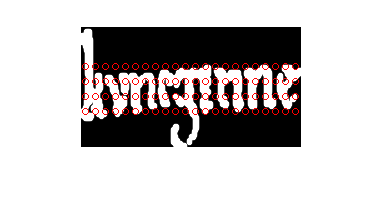
\includegraphics[width=0.5\textwidth]{descriptor_placement}
\caption{Placement of SFIT descriptors on a regular grid.}
\label{fig:SIFT}
\end{figure}

\subsection{Words}
\label{sub:words}
Since SIFT descriptors have a quite high dimensionality (every is a vector with 128 components)
and our sampling is quite dense (88 descriptors for Figure \ref{SIFT}), we condense the
descriptor using the bag of words technique. 

For this purpose, we cluster the all descriptors retrieved from the database using k-means to
50 clusters. Then we segment the image vertically into slots and count the number of words 
in each slot. This gives us a histogram with 50 bins for every slot, that we concatenate to one
big structure representing an image (See Figure \ref{fig:histogram}).
\begin{figure}[!t]
\centering
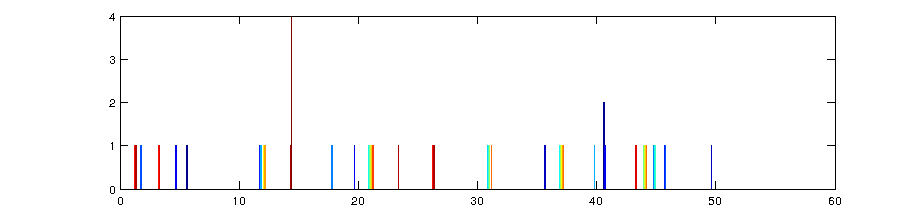
\includegraphics[width=0.5\textwidth]{kvniginne_histogram}
\caption{The concatenated histogram of words for the image from Figure \ref{SIFT}.}
\label{fig:histogram}
\end{figure}
% subsection words (end)

\subsection{Computing similarities}
\label{sub:similarities}
For computing the similarity between a query image and a database image, 
we compare their histograms. While other authors have proven that dynamic time warping can be
used effectively for this in keyword spotting, we did not have any success with it. We ended
up just trying to match the query image $q$ 
at every possible offset $o$ of a database image $d$, then taking
the minimum over all possibilities.
 For a given offset, we compute the distance as L2 norm over all slots.
\begin{equation}
	dist(d, q) = \min_o \sum_{i \in S} || d_{i + o} - q_{i}  ||_2
\end{equation}

% subsection similarities (end)

\subsection{User interaction}
\label{sub:user interaction}
We expect a user query to be of the form "Retrieve the n most similar image to the given query
image". Using our distance measure defined above, 
we create a ranking and return the top n entries.
% subsection user interaction (end)

\section{Results}
While our keyword spotting framework achieved very promising results in some cases, when matching single words (See e.g. Figure \ref{fig:results_words:roxx}), very short words (Figure \ref{fig:results_words:suxx}) were troublesome until the very end. Additional results are depicted in figure $\ref{fig:Results_nice2}$.

Unfortunately, the results for the short words worsened as we tried to generalize our method for finding keywords in full sentences instead of
matching only words.
\begin{figure}[ht!]%
\centering
\subfigure[A-r-t-v-s EER=0.941176]{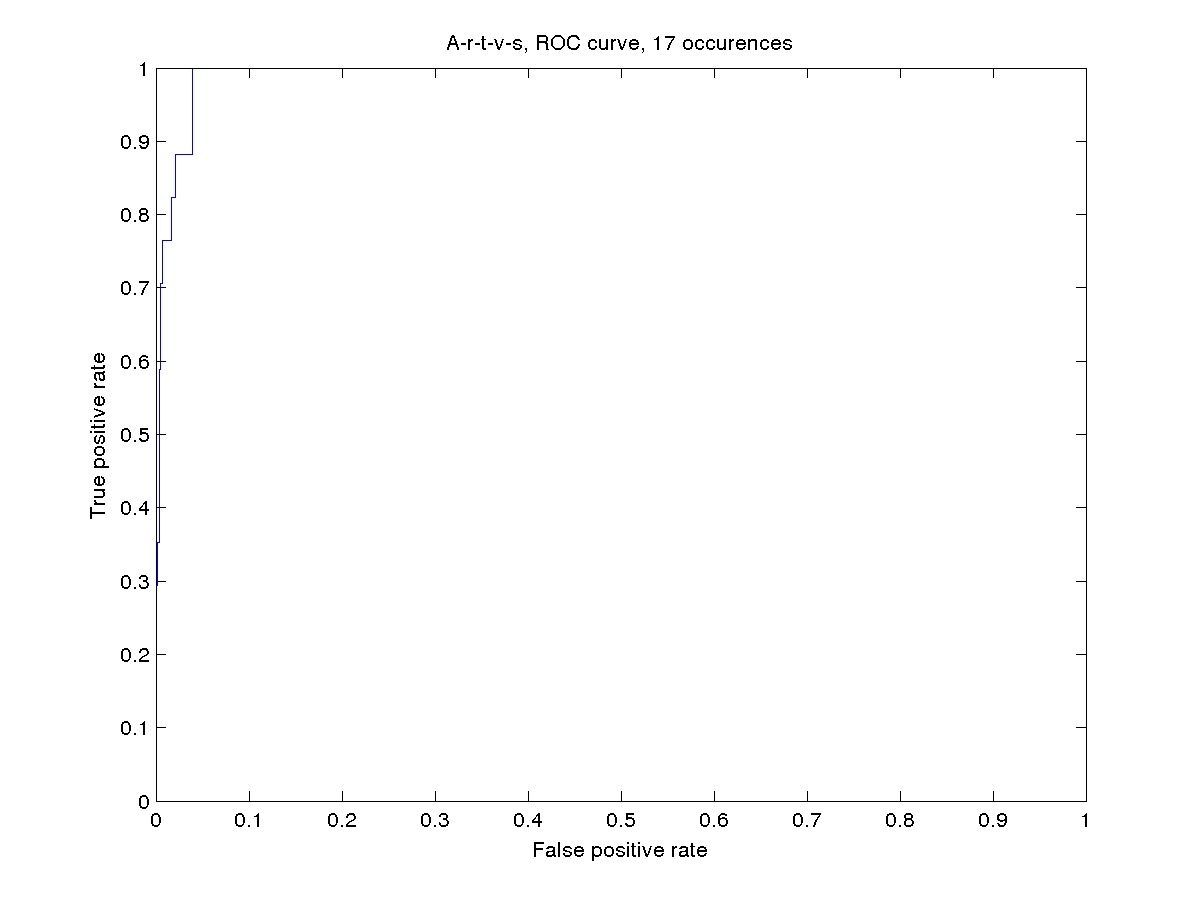
\includegraphics[width=0.23\textwidth]{A-r-t-v-s_roc}}
\subfigure[G-r-a-l-s EER=0.875000]{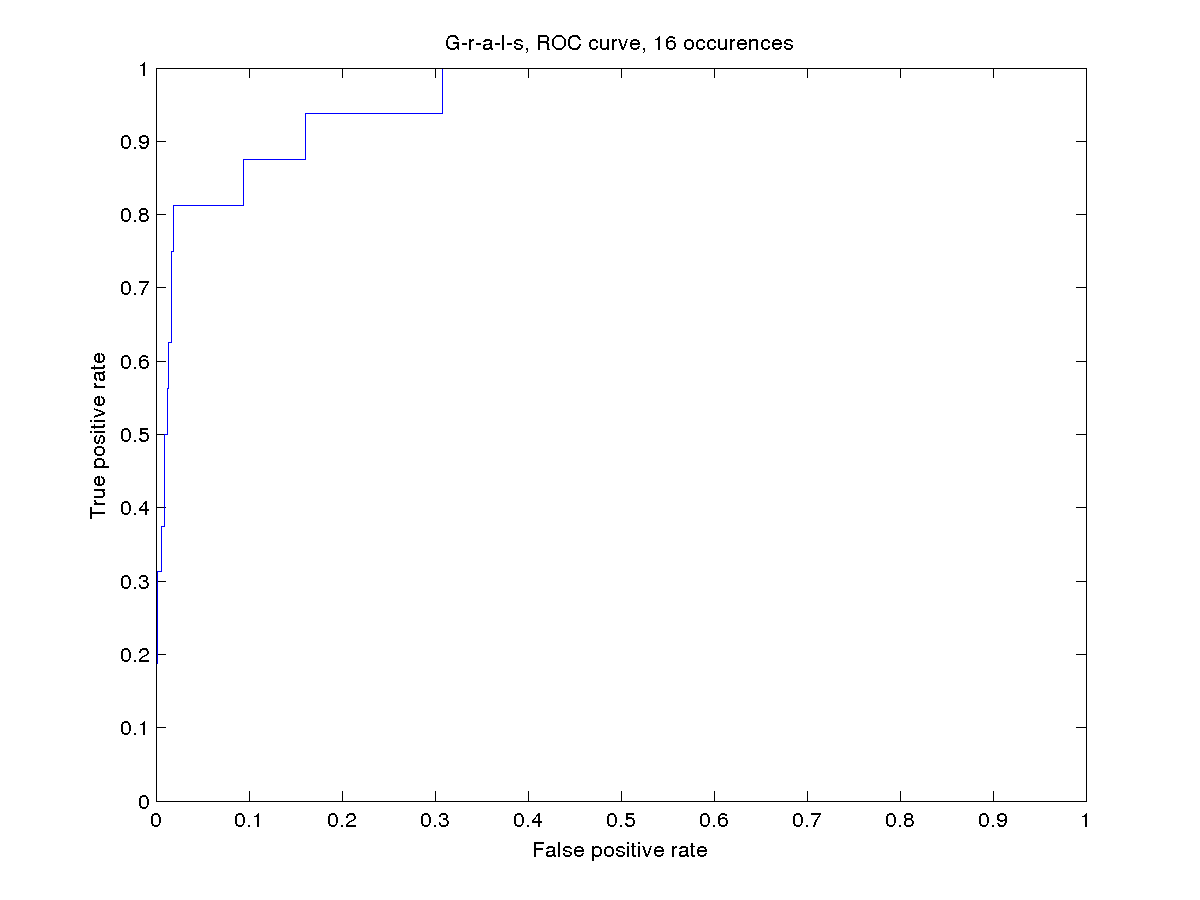
\includegraphics[width=0.23\textwidth]{G-r-a-l-s_roc}}\\
\subfigure[d-a-z EER=0.201493]{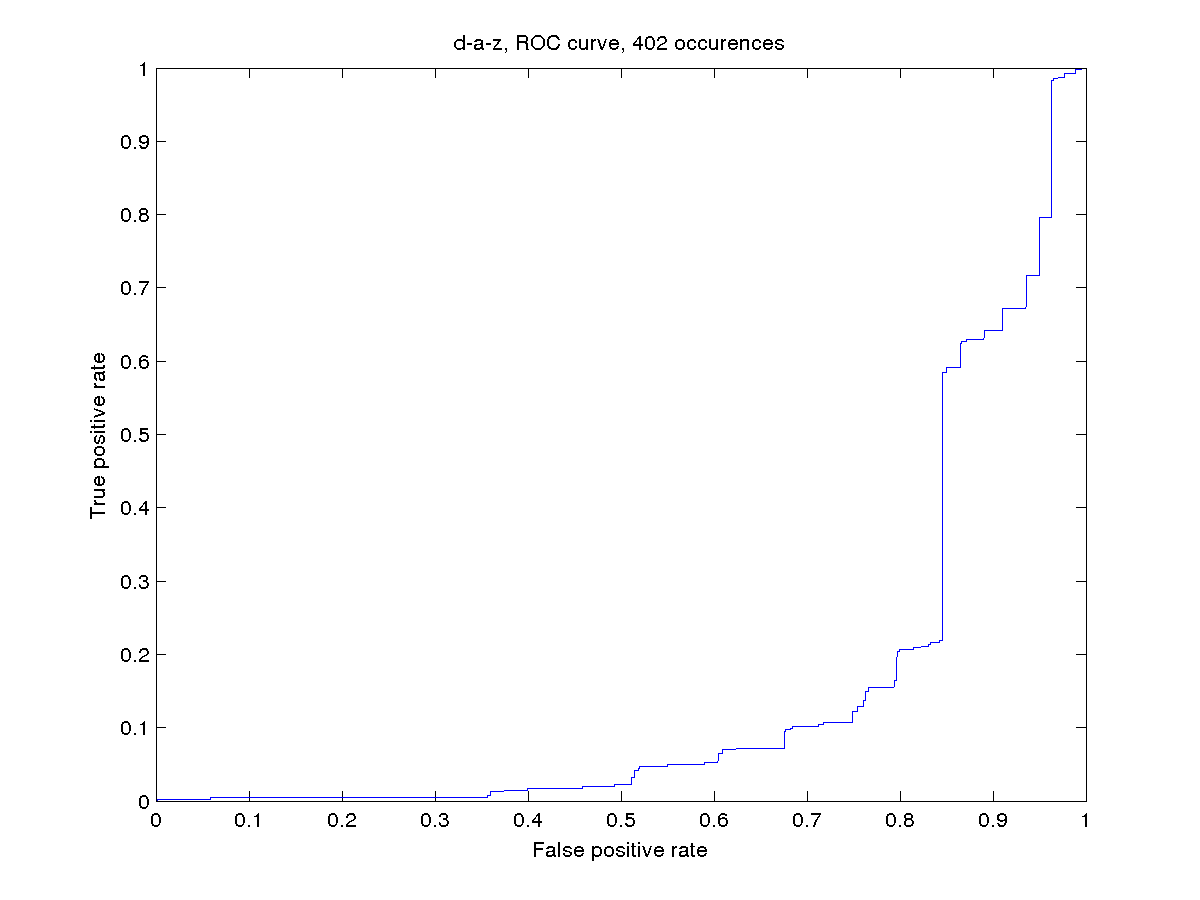
\includegraphics[width=0.23\textwidth]{d-a-z_roc}
\label{fig:results_words:suxx}}
\subfigure[k-v-n-e-g-i-n-n-e EER=1.000000]{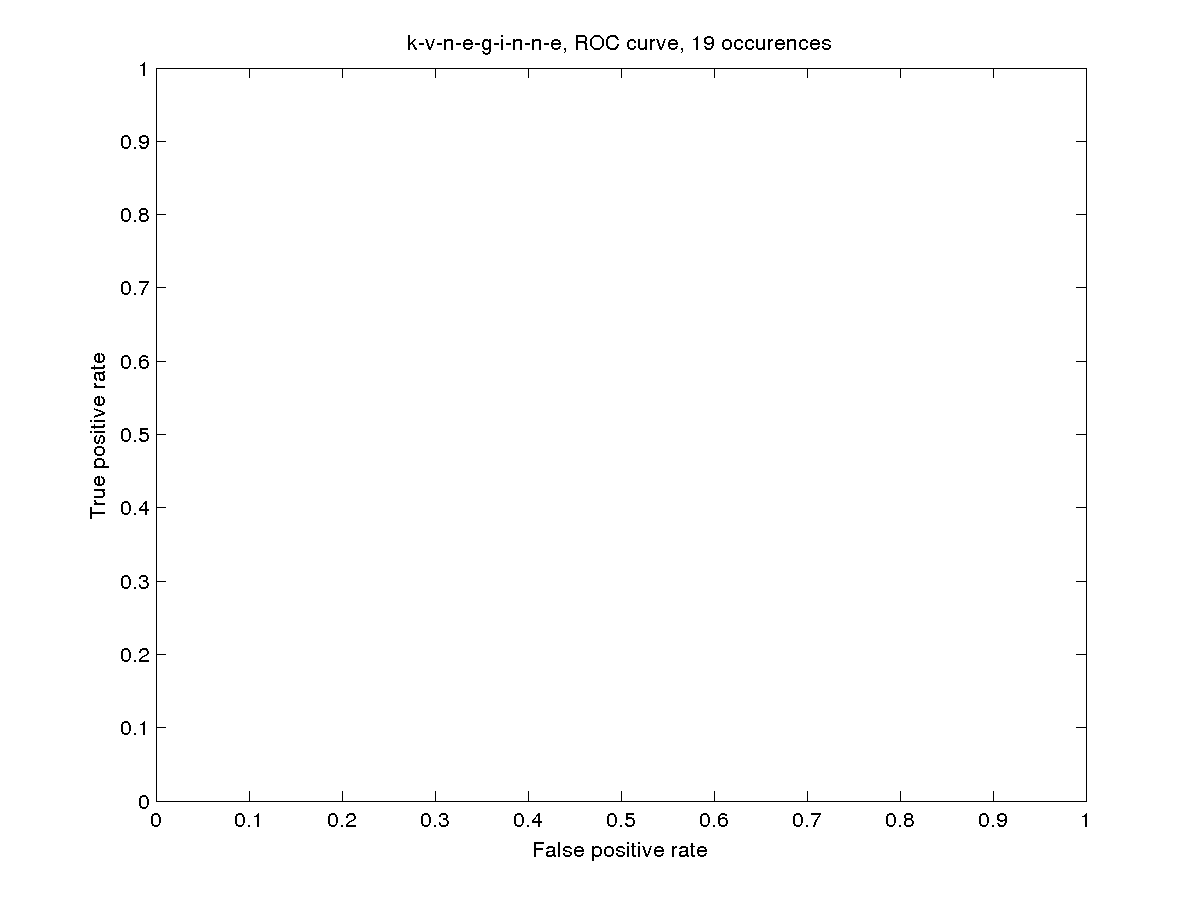
\includegraphics[width=0.23\textwidth]{k-v-n-e-g-i-n-n-e_roc}
\label{fig:results_words:roxx}}
\caption{ROC graphs when matching single words.}
\label{fig:Results}
\end{figure}
\begin{figure}[ht!]%
\centering
\subfigure[A-r-t-v-s AP=0.638034]{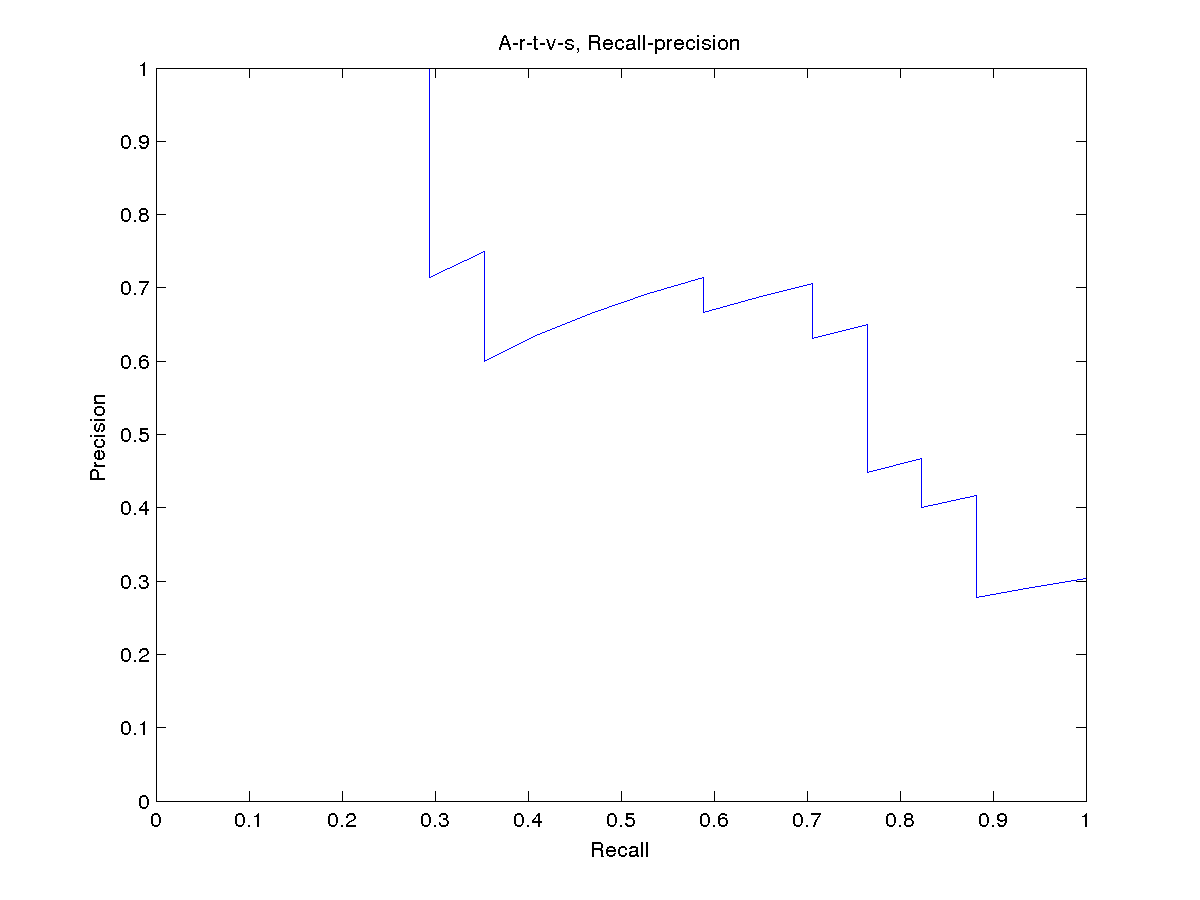
\includegraphics[width=0.23\textwidth]{A-r-t-v-s_rp}}
\subfigure[G-r-a-l-s AP=0.418035]{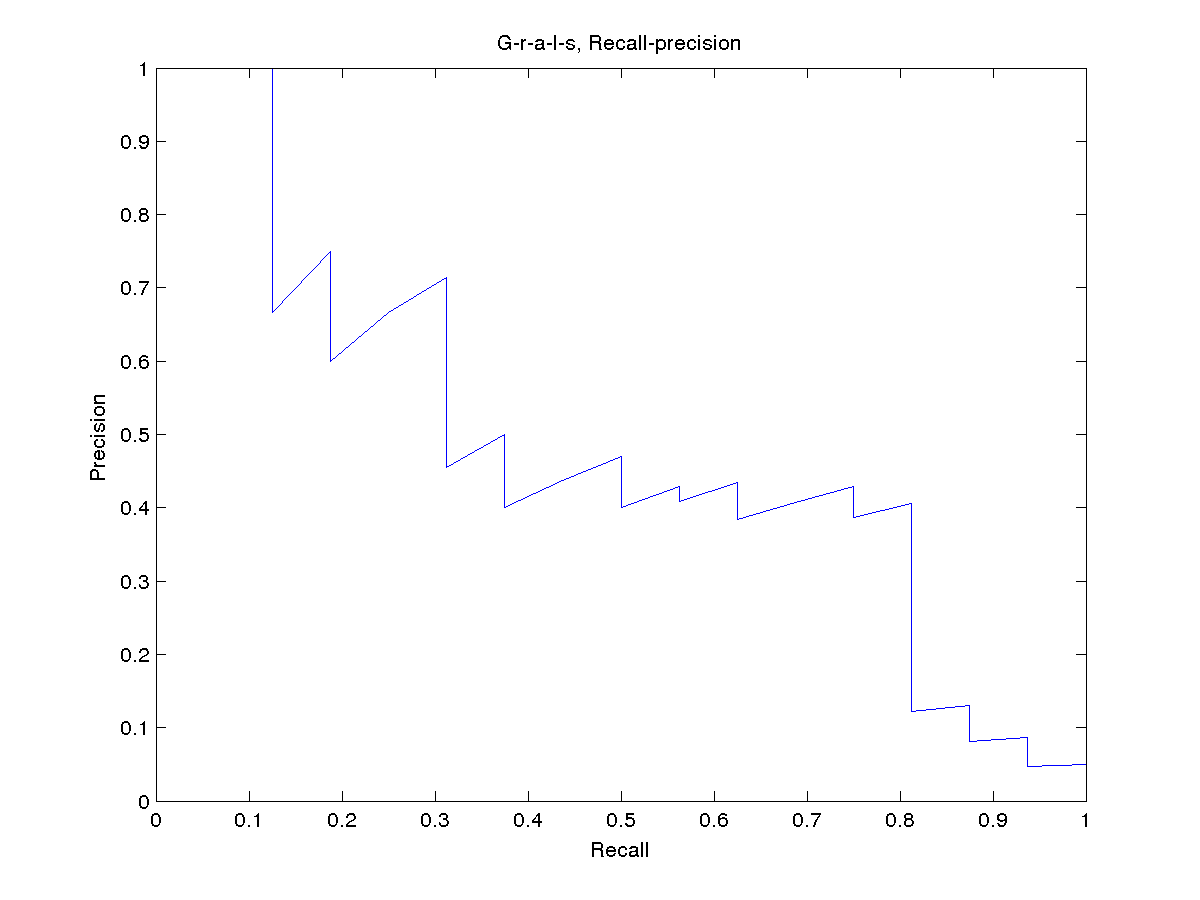
\includegraphics[width=0.23\textwidth]{G-r-a-l-s_rp}}\\
\subfigure[d-a-z AP=0.256762]{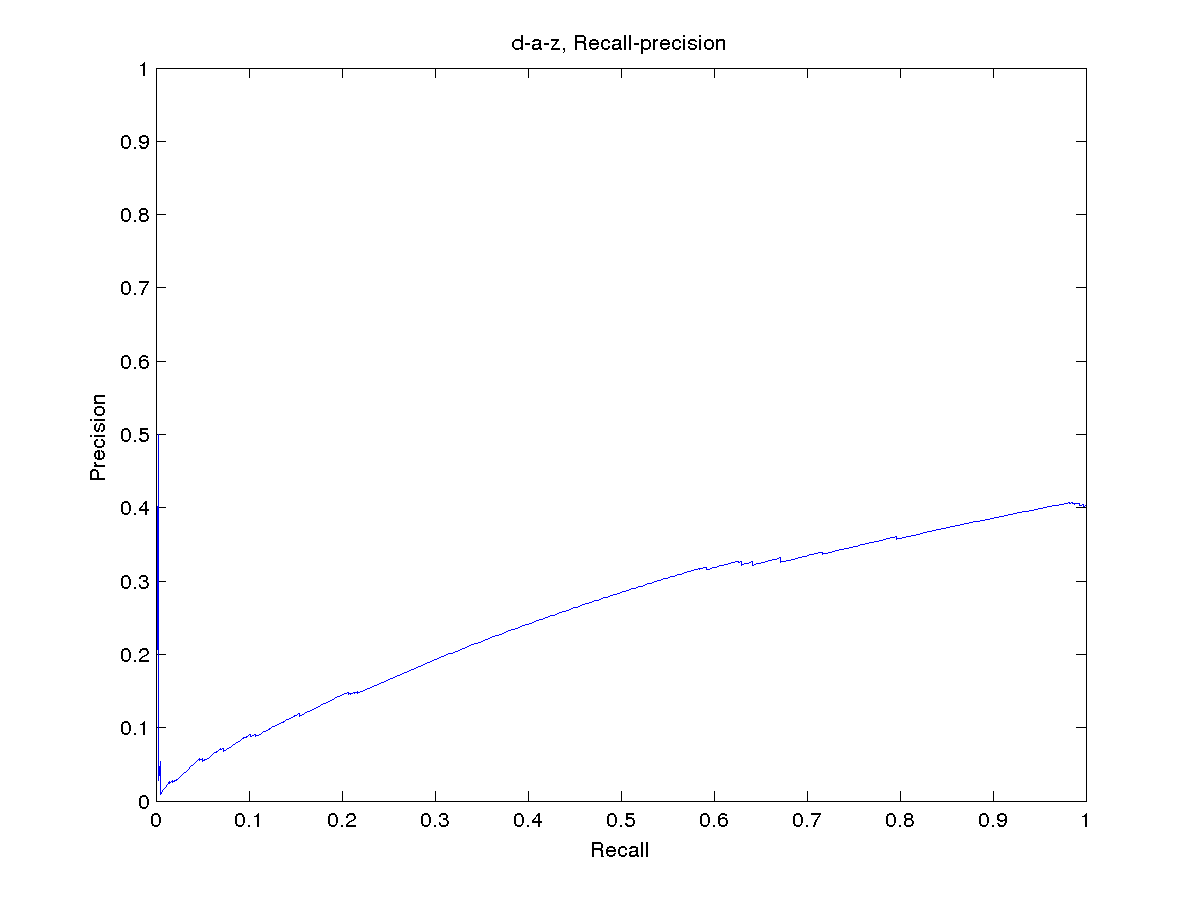
\includegraphics[width=0.23\textwidth]{d-a-z_rp}}
\subfigure[k-v-n-e-g-i-n-n-e AP=1.000000]{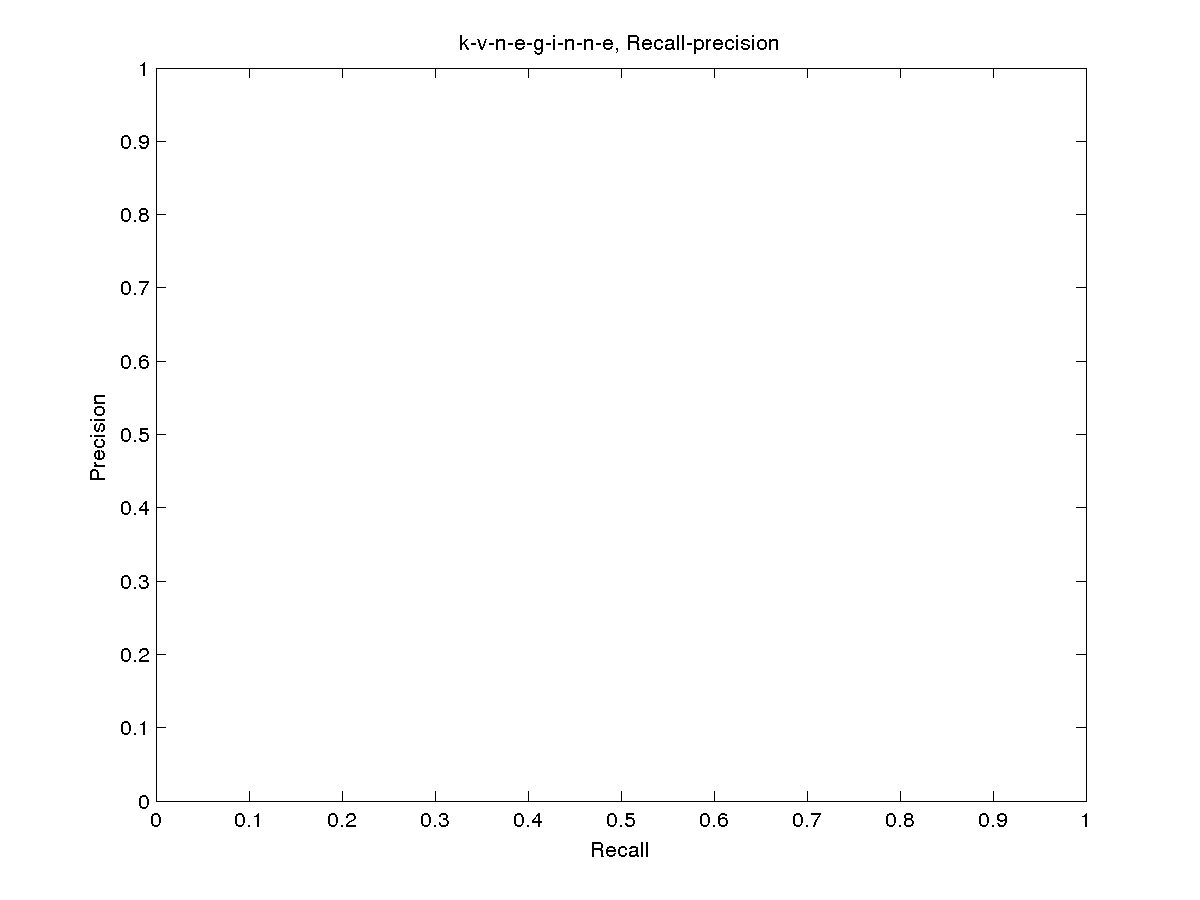
\includegraphics[width=0.23\textwidth]{k-v-n-e-g-i-n-n-e_rp}}
\caption{Recall-Precision graphs when matching single words.}
\label{fig:Results_nice2}
\end{figure}

When querying full sentences with a keyword, however, 
our method does unfortunately not yield satisfying results. The quality of our algorithm for matching a query words in sentences is illustrated in figure $\ref{fig:Results}$ and in figure $\ref{fig:Results_sentences}$.
\begin{figure}[ht!]%
\centering
\subfigure[A-r-t-v-s EER=0.647059]{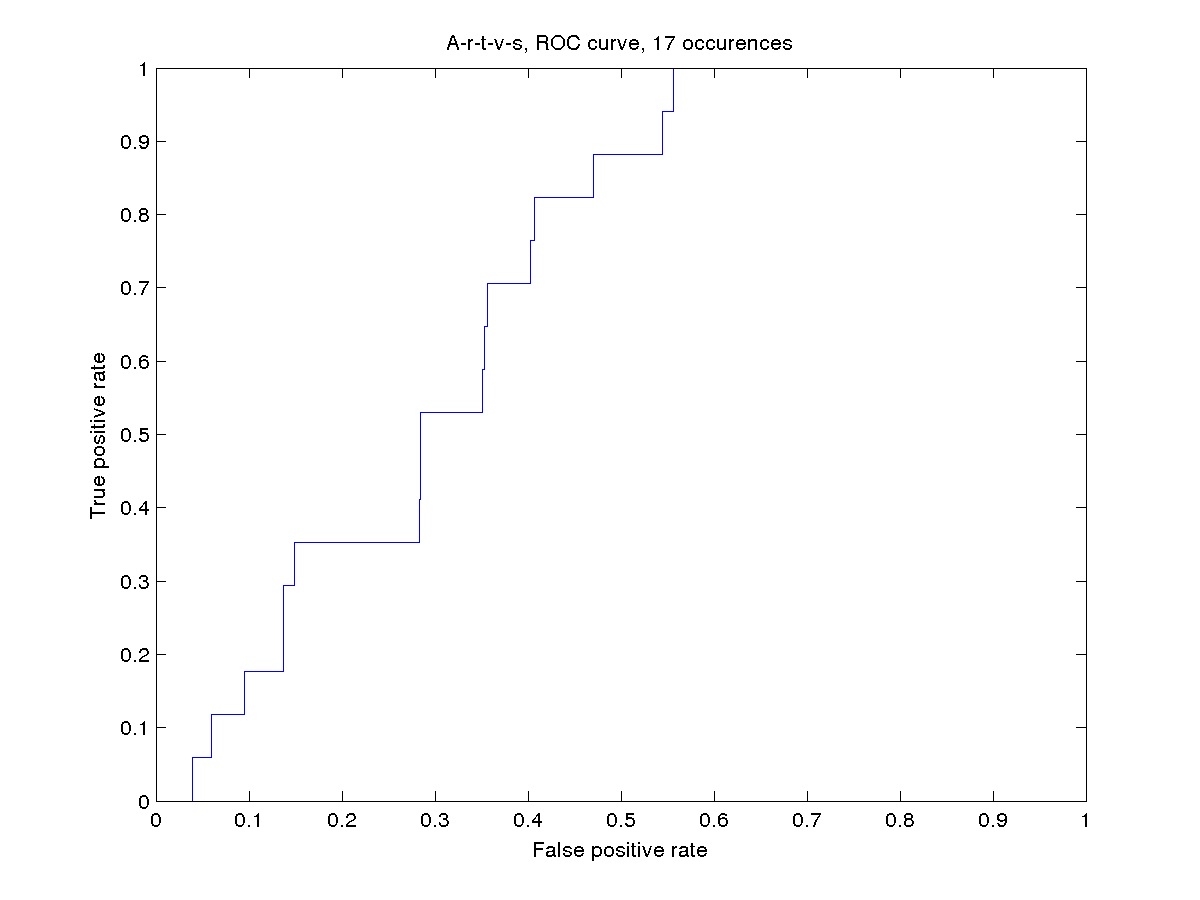
\includegraphics[width=0.23\textwidth]{A-r-t-v-s_sent_roc}}
\subfigure[G-r-a-l-s EER=0.375000]{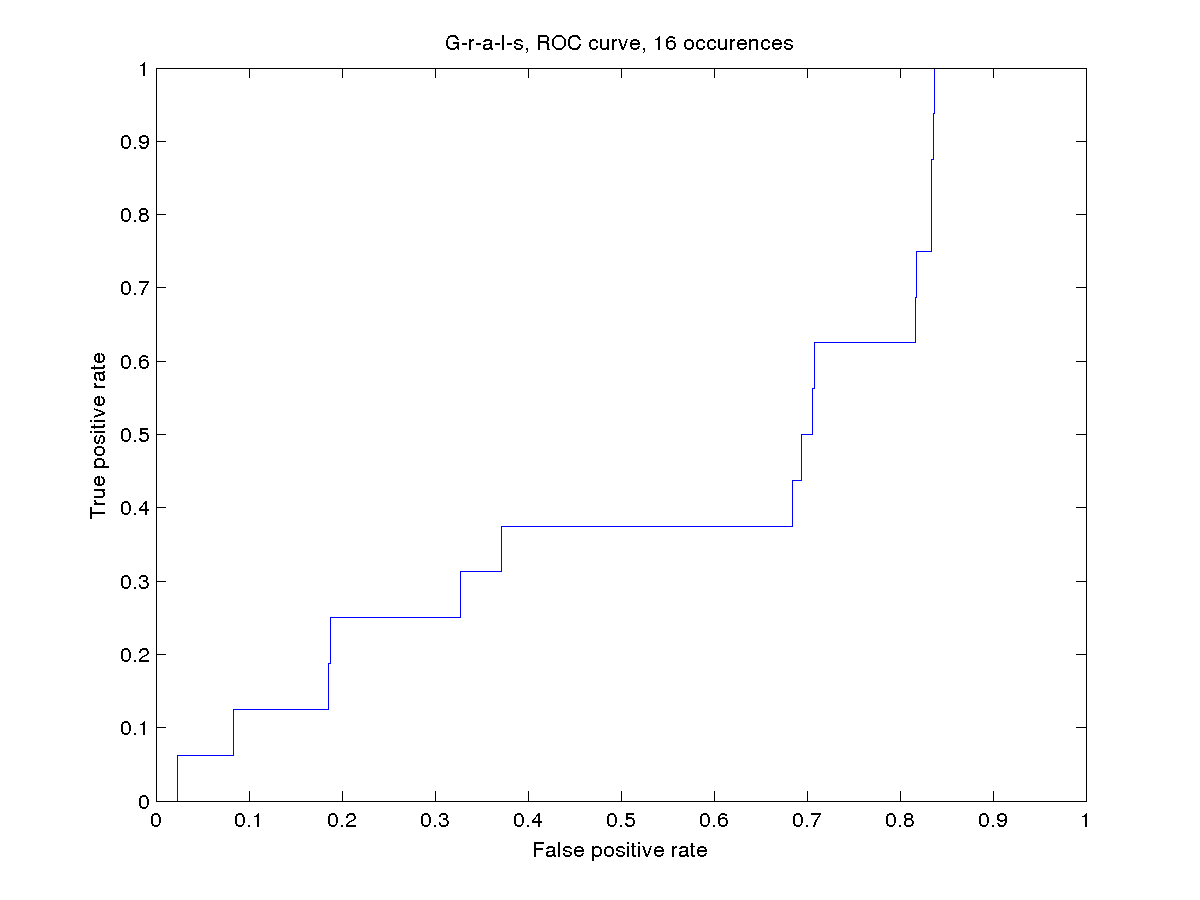
\includegraphics[width=0.23\textwidth]{G-r-a-l-s_sent_roc}}\\
\subfigure[d-a-z EER=0.0.405542]{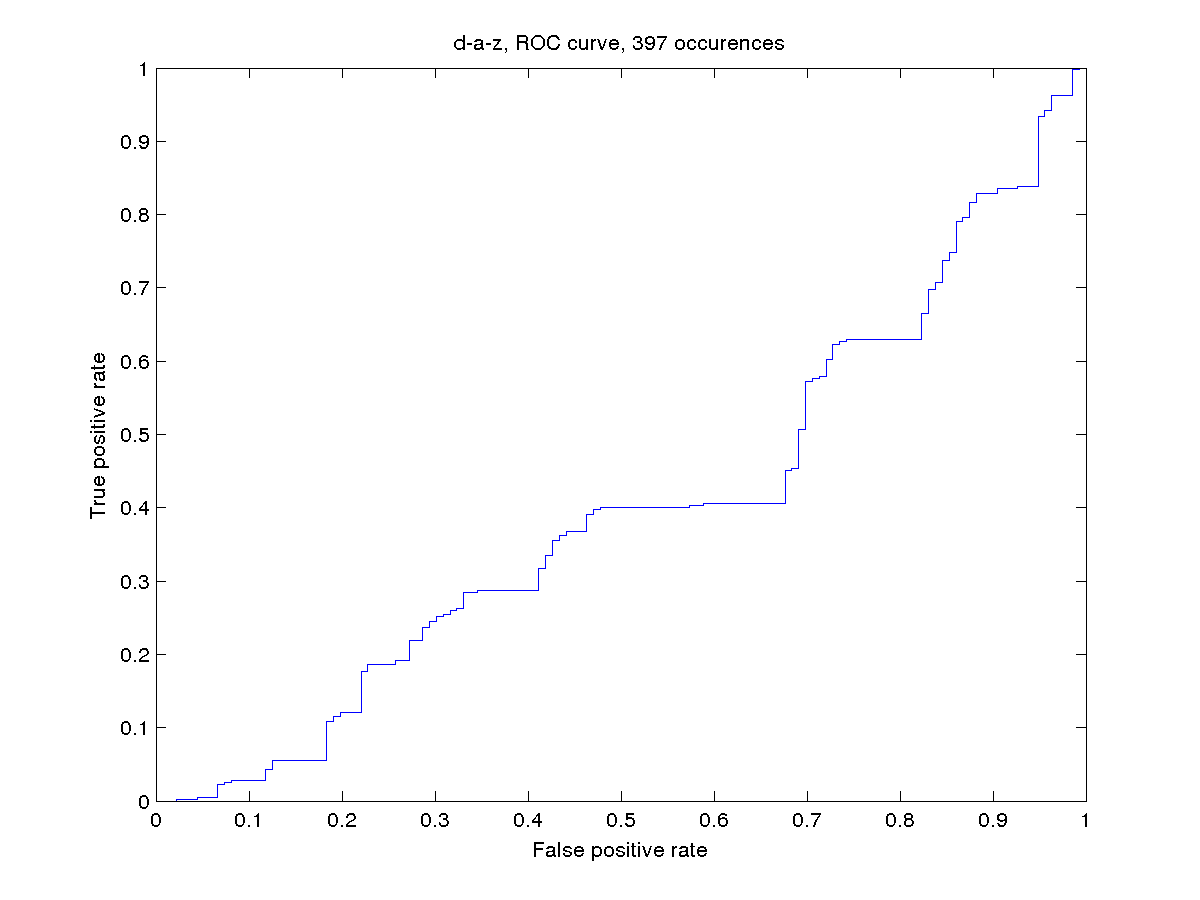
\includegraphics[width=0.23\textwidth]{d-a-z_sent_roc}}
\subfigure[k-v-n-e-g-i-n-n-e EER=0.631579]{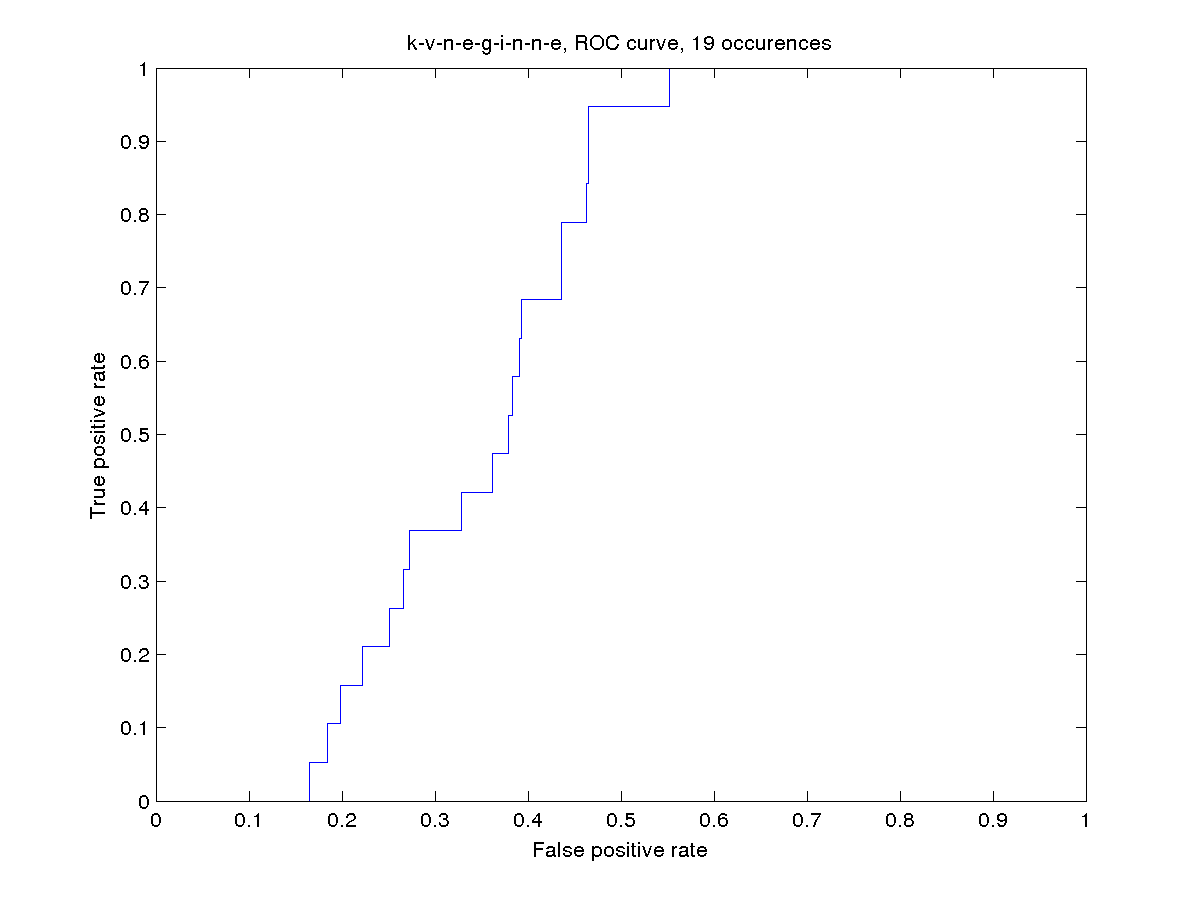
\includegraphics[width=0.23\textwidth]{k-v-n-e-g-i-n-n-e_sent_roc}}
\caption{ROC graphs when matching full sentences.}
\label{fig:Results}
\end{figure}

\begin{figure}[ht!]%
\centering
\subfigure[A-r-t-v-s AP=0.051786]{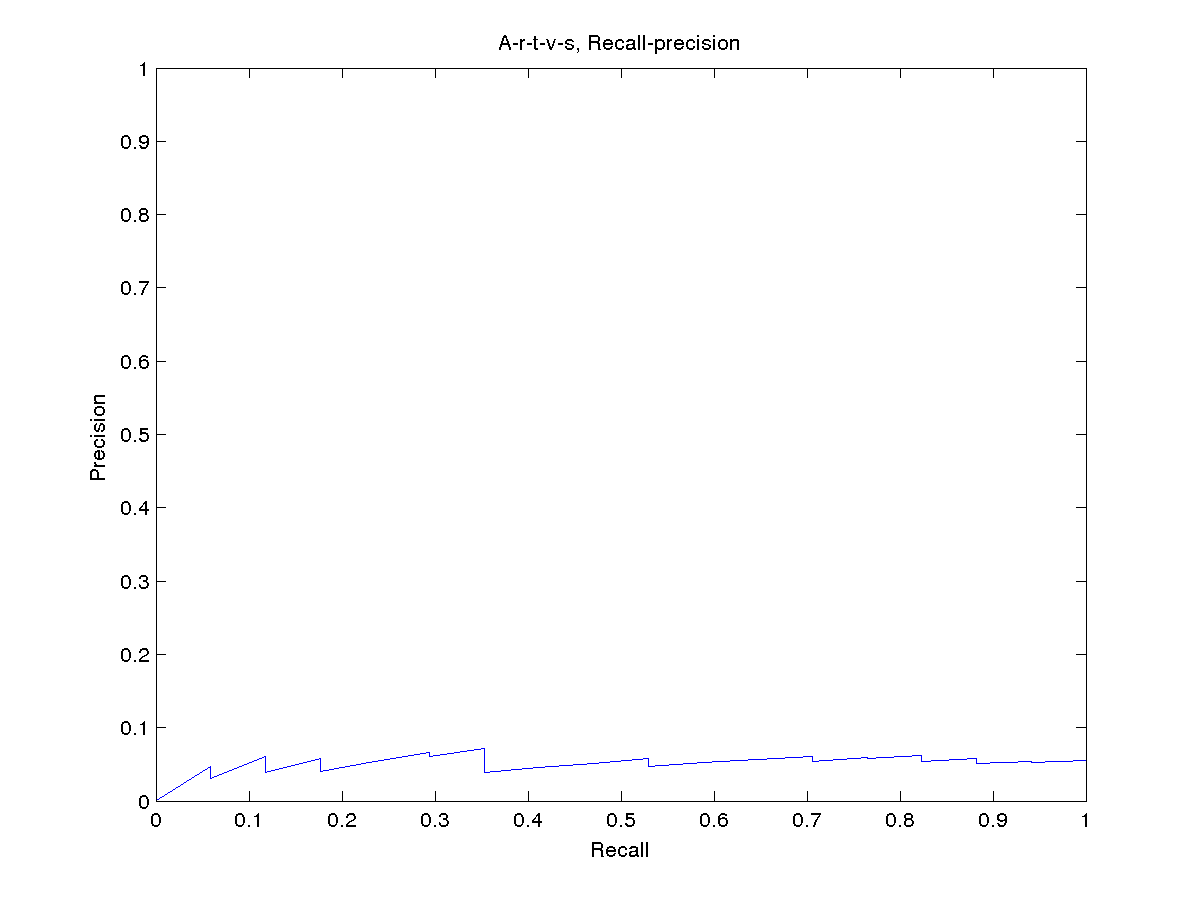
\includegraphics[width=0.23\textwidth]{A-r-t-v-s_sent_rp}}
\subfigure[G-r-a-l-s AP=0.028053]{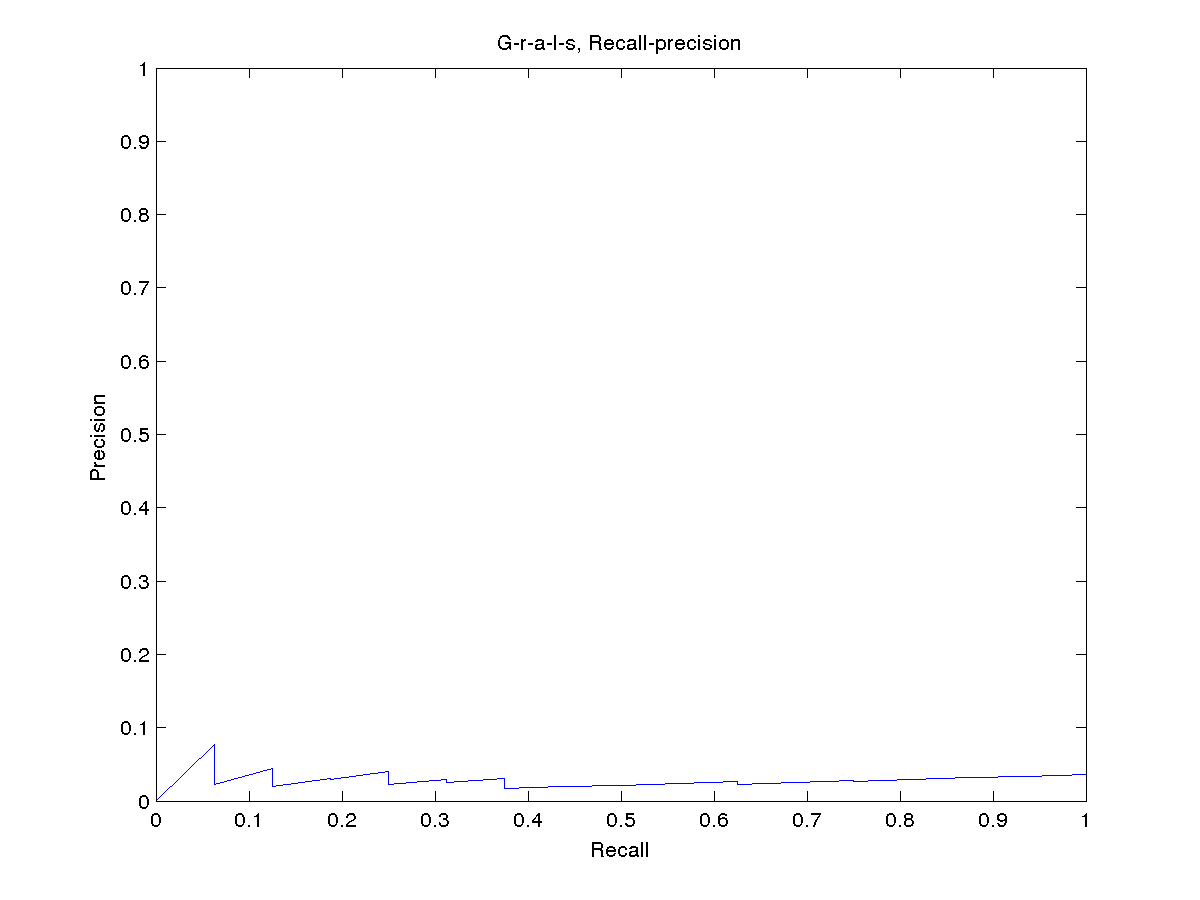
\includegraphics[width=0.23\textwidth]{G-r-a-l-s_sent_rp}}\\
\subfigure[d-a-z AP=0.678544]{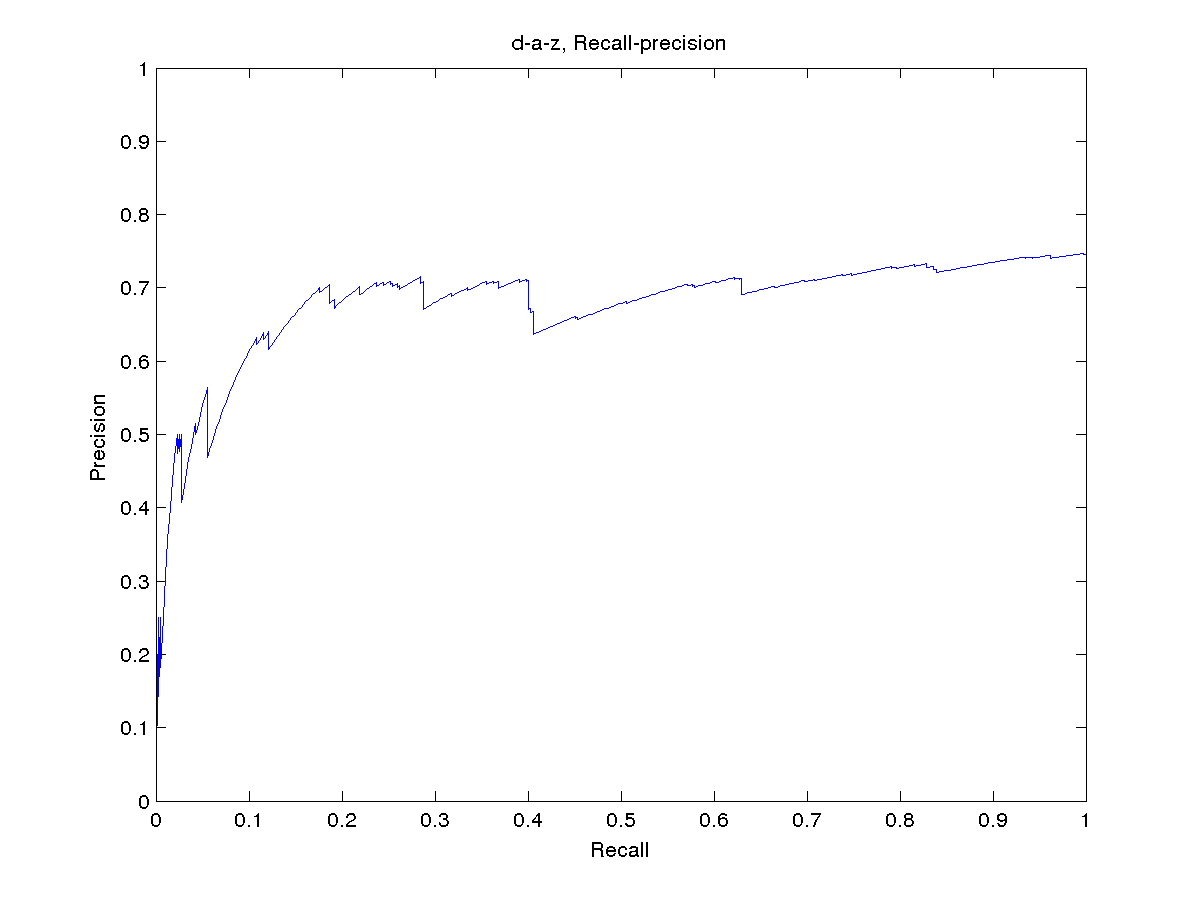
\includegraphics[width=0.23\textwidth]{d-a-z_sent_rp}}
\subfigure[k-v-n-e-g-i-n-n-e AP=0.045262]{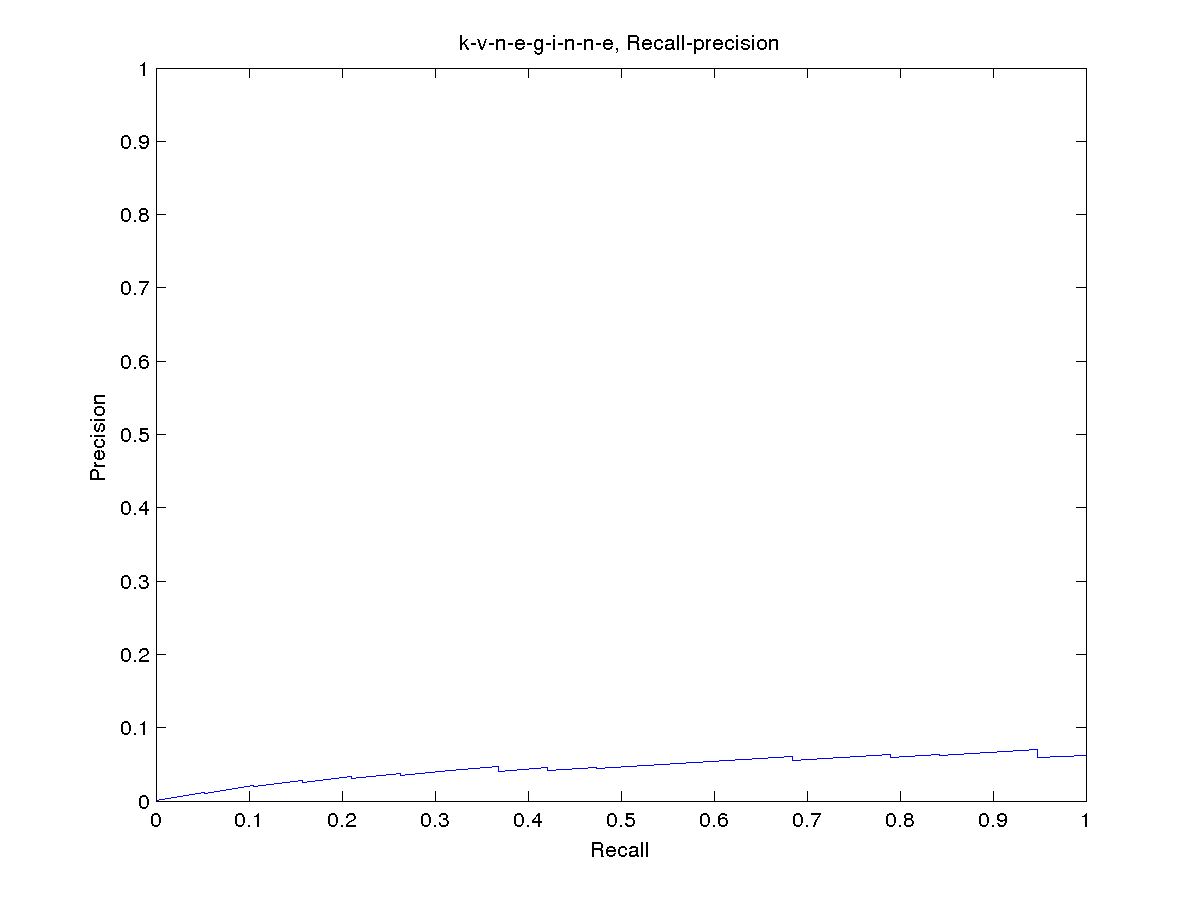
\includegraphics[width=0.23\textwidth]{k-v-n-e-g-i-n-n-e_sent_rp}}
\caption{Recall-Precision graphs when matching full sentences.}
\label{fig:Results_sentences}
\end{figure}

\section{Conclusion}
In this work we developed and discussed a method how to detect keywords in handwritten document. The underlying idea of our approach is based on SIFT feature extraction and a bog of words approach. The reason for following such an approach was that we wanted to invariant to the orientation, scale, position of the historical documents. 

Referring to our findings in the result section we observe that our approach performs rather well for detecting visual query words in a word database. However, when we try to spot query-keywords in a visual sentence database our current algorithm the performance of our algorithm is rather poor. This last finding seems somewhat counterintuitive since from our point of view SIFT features ensure different types of invariances. 

Since all words in the visual word database are normalized we suppose that this helped our algorithm to achieve its good performance whereas the sentence database is not normalized. Thus the second task does not yield equally well results when running our algorithm. Furthermore, we also thought of the possibility that SIFT is not the appropriate choice of feature descriptor for detecting handwritten words visual sentences. 


% An example of a floating figure using the graphicx package.
% Note that \label must occur AFTER (or within) \caption.
% For figures, \caption should occur after the \includegraphics.
% Note that IEEEtran v1.7 and later has special internal code that
% is designed to preserve the operation of \label within \caption
% even when the captionsoff option is in effect. However, because
% of issues like this, it may be the safest practice to put all your
% \label just after \caption rather than within \caption{}.
%
% Reminder: the "draftcls" or "draftclsnofoot", not "draft", class
% option should be used if it is desired that the figures are to be
% displayed while in draft mode.
%
%\begin{figure}[!t]
%\centering
%\includegraphics[width=2.5in]{myfigure}
% where an .eps filename suffix will be assumed under latex, 
% and a .pdf suffix will be assumed for pdflatex; or what has been declared
% via \DeclareGraphicsExtensions.
%\caption{Simulation Results}
%\label{fig_sim}
%\end{figure}

% Note that IEEE typically puts floats only at the top, even when this
% results in a large percentage of a column being occupied by floats.


% An example of a double column floating figure using two subfigures.
% (The subfig.sty package must be loaded for this to work.)
% The subfigure \label commands are set within each subfloat command, the
% \label for the overall figure must come after \caption.
% \hfil must be used as a separator to get equal spacing.
% The subfigure.sty package works much the same way, except \subfigure is
% used instead of \subfloat.
%
%\begin{figure*}[!t]
%\centerline{\subfloat[Case I]\includegraphics[width=2.5in]{subfigcase1}%
%\label{fig_first_case}}
%\hfil
%\subfloat[Case II]{\includegraphics[width=2.5in]{subfigcase2}%
%\label{fig_second_case}}}
%\caption{Simulation results}
%\label{fig_sim}
%\end{figure*}
%
% Note that often IEEE papers with subfigures do not employ subfigure
% captions (using the optional argument to \subfloat), but instead will
% reference/describe all of them (a), (b), etc., within the main caption.


% An example of a floating table. Note that, for IEEE style tables, the 
% \caption command should come BEFORE the table. Table text will default to
% \footnotesize as IEEE normally uses this smaller font for tables.
% The \label must come after \caption as always.
%
%\begin{table}[!t]
%% increase table row spacing, adjust to taste
%\renewcommand{\arraystretch}{1.3}
% if using array.sty, it might be a good idea to tweak the value of
% \extrarowheight as needed to properly center the text within the cells
%\caption{An Example of a Table}
%\label{table_example}
%\centering
%% Some packages, such as MDW tools, offer better commands for making tables
%% than the plain LaTeX2e tabular which is used here.
%\begin{tabular}{|c||c|}
%\hline
%One & Two\\
%\hline
%Three & Four\\
%\hline
%\end{tabular}
%\end{table}


% Note that IEEE does not put floats in the very first column - or typically
% anywhere on the first page for that matter. Also, in-text middle ("here")
% positioning is not used. Most IEEE journals/conferences use top floats
% exclusively. Note that, LaTeX2e, unlike IEEE journals/conferences, places
% footnotes above bottom floats. This can be corrected via the \fnbelowfloat
% command of the stfloats package.


% trigger a \newpage just before the given reference
% number - used to balance the columns on the last page
% adjust value as needed - may need to be readjusted if
% the document is modified later
%\IEEEtriggeratref{8}
% The "triggered" command can be changed if desired:
%\IEEEtriggercmd{\enlargethispage{-5in}}

\bibliographystyle{IEEEtran}
\bibliography{IEEEabrv,report}
\end{document}

